\documentclass[10pt]{scrartcl}

% \usepackage{auto1}
% \usepackage[T1]{fontenc}
% \usepackage{MinionPro}
% \usepackage{MyriadPro}
\renewcommand{\familydefault}{\sfdefault}

% \usepackage{beramono}

\usepackage[eso-foot]{svninfo}

\usepackage[margin=0.5in]{geometry}

\usepackage{tabularx}
\usepackage{booktabs}

\usepackage{tikz}
\usetikzlibrary{shapes}
\usetikzlibrary{arrows}
\usetikzlibrary{decorations}

\usepackage{fancyvrb}

\pagestyle{empty}


\newcommand{\ttffile}{\texttt{\$TTF\_FILE}}
\newcommand{\encfile}{\texttt{\$ENC\_FILE}}

\newcommand{\sample}{
\begin{tabular}{p{2.5ex}@{}p{2.5ex}@{}p{2.5ex}@{}p{2.5ex}@{}p{2.5ex}@{}p{2.5ex}@{}p{2.5ex}@{}p{2.5ex}@{}p{2.5ex}@{}p{2.5ex}@{}p{2.5ex}@{}p{2.5ex}@{}p{2.5ex}@{}p{2.5ex}@{}p{2.5ex}}
0 & 1 & 2 & 3 & 4 & 5 & 6 & 7 & 9 &   &\\
a & b & c & d & e & f & g & h & i & j & k & l & m & n\\
o & p & q & r & s & t & u & v & w & x & y & z\\
A & B & C & D & E & F & G & H & I & J & K & L & M & N\\
O & P & Q & R & S & T & U & V & W & X & Y & Z
\end{tabular}%
% {0}{1}{2}{3}{4}{5}{6}{7}{8}{9}\\
% {a}{b}{c}{d}{e}{f}{g}{h}{i}{j}{k}{l}{m}{n}{o}{p}{q}{r}{s}{t}{u}{v}{w}{x}{y}{z}\\
% {A}{B}{C}{D}{E}{F}{G}{H}{I}{J}{K}{L}{M}{N}{O}{P}{Q}{R}{S}{T}\\
% {U}{V}{W}{X}{Y}{Z}
}

\begin{document}

\centering

% ============================================================================
% END 1st page
% ============================================================================
\section*{{\TeX} font errors: Cheatsheet}

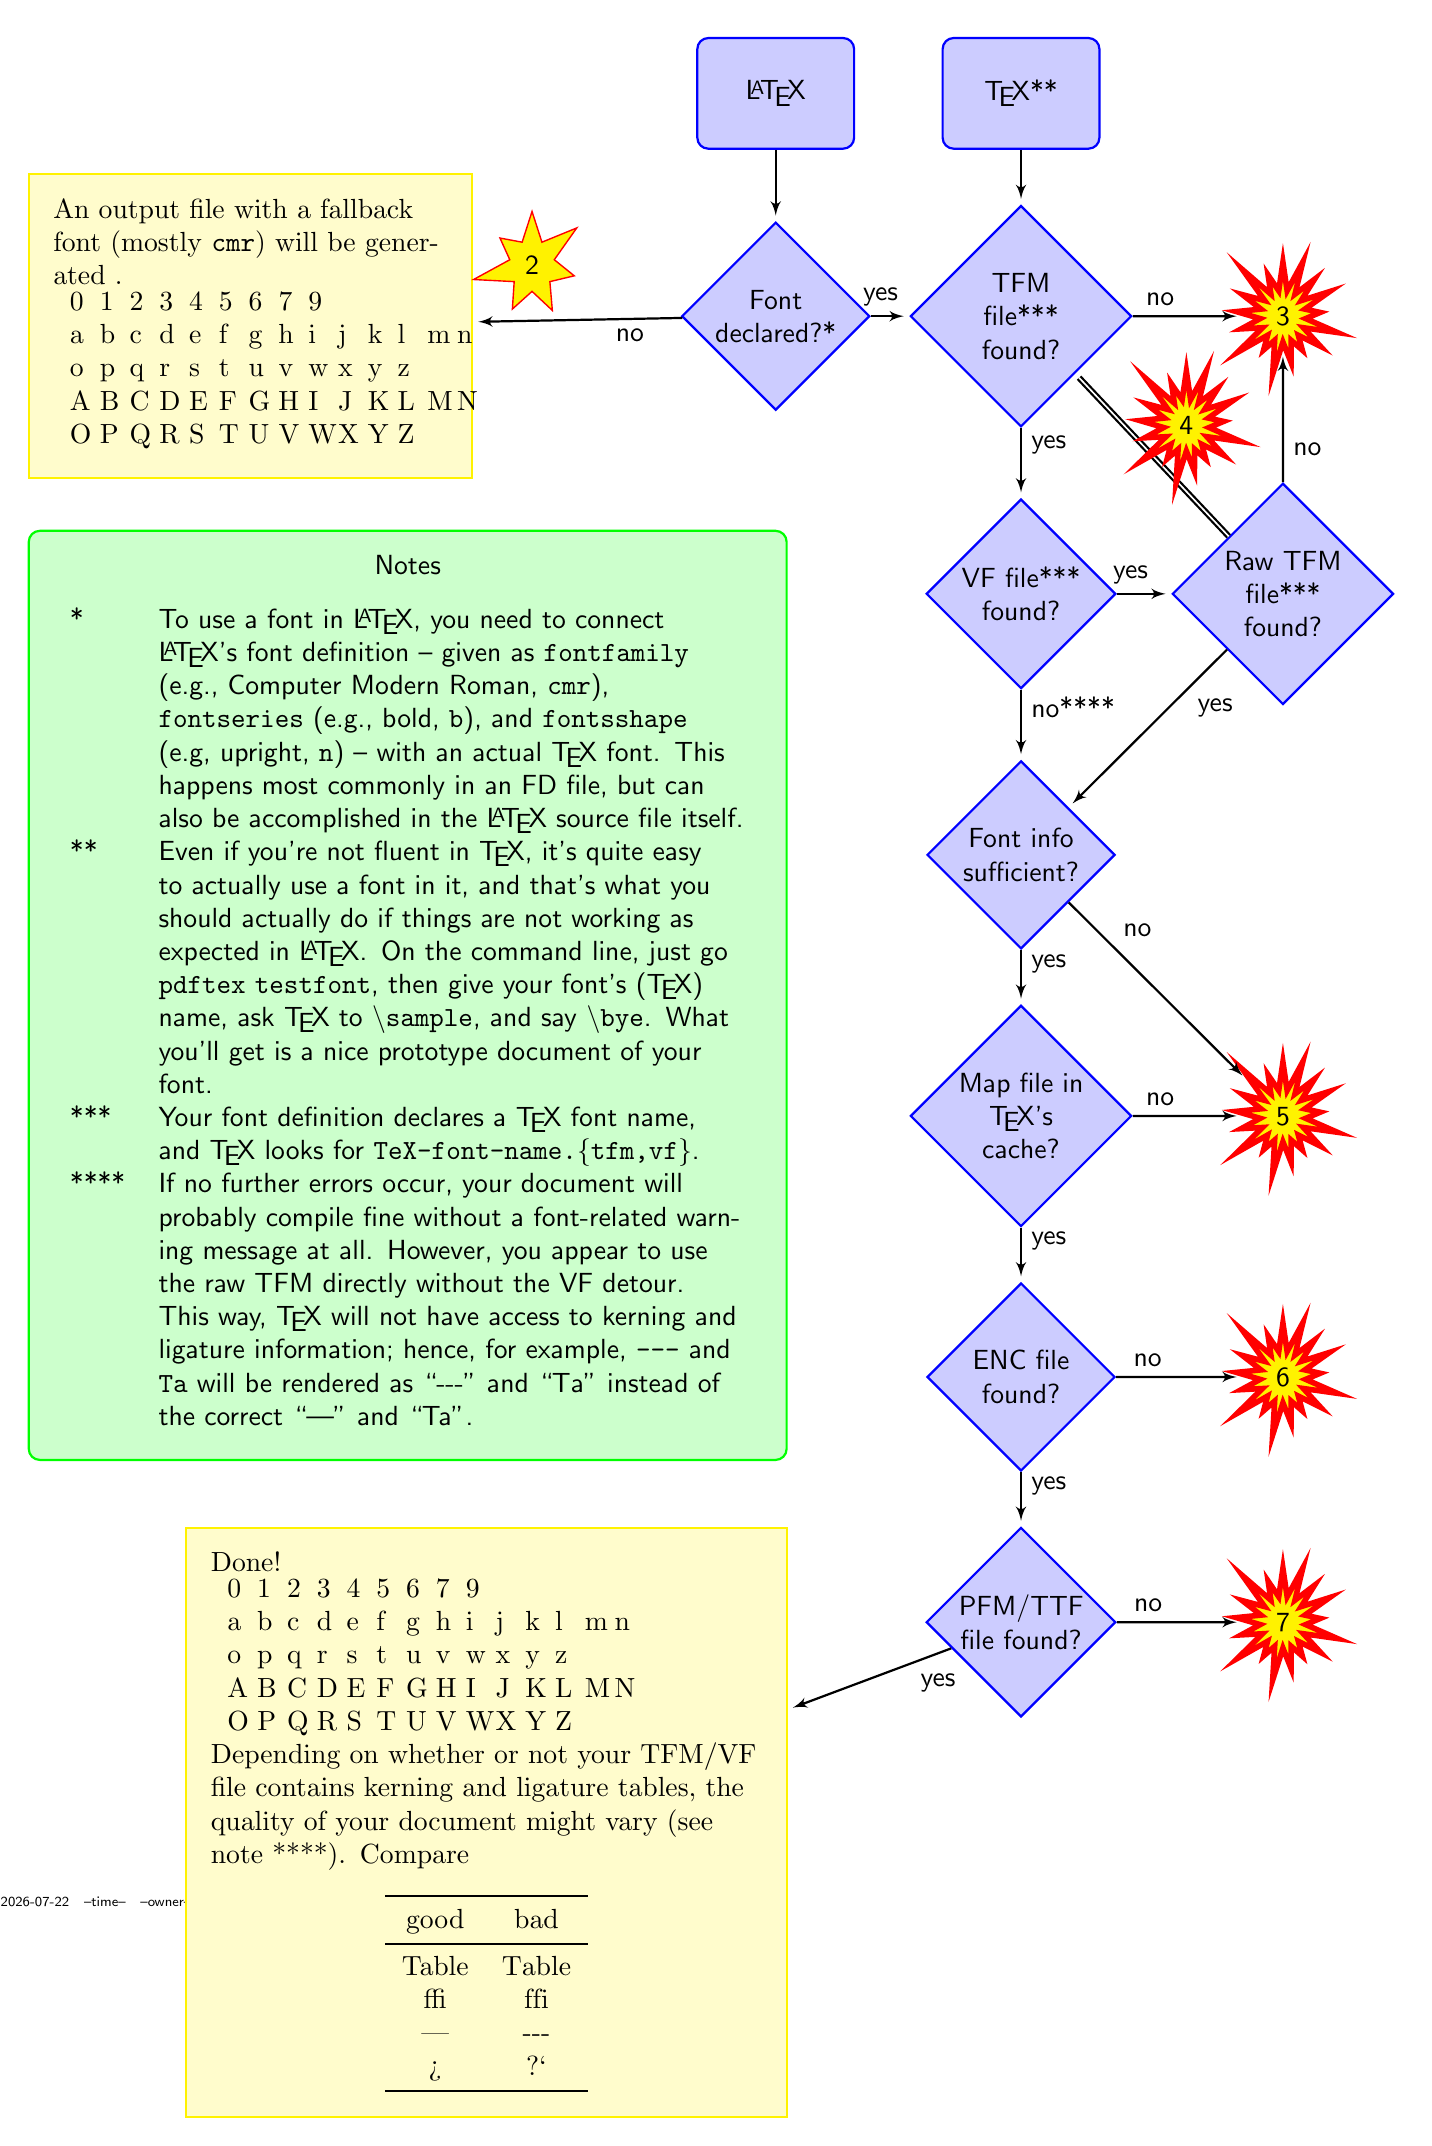
\begin{tikzpicture}
[auto,
decision/.style = {diamond, draw=blue, thick, fill=blue!20, text width=4.5em, text badly centered,inner sep=1pt},
block/.style    = {rectangle, draw=blue, thick, fill=blue!20, text width=5em, text centered, rounded corners, minimum height=4em},
line/.style     = {draw, thick, -latex',shorten >=2pt},
error/.style    = {draw=red, thick, fill=red!20, minimum height=2em},
error_number/.style  = {starburst, fill=yellow, draw=red, line width=2pt,starburst points=17},
warning_number/.style  = {starburst, fill=yellow, draw=red, line width=0.5pt,starburst points=7},
output/.style   = {draw=yellow, thick, fill=yellow!20, text width=5cm,minimum height=2em, inner sep=2ex}
]

% \node[starburst, fill=yellow, draw=red, line width=2pt] {\bf BANG!};

% - - - - - - - - - - - - - - - - - - - - - - - - - - - - - - - - - - - - - -
% *** matrix
% - - - - - - - - - - - - - - - - - - - - - - - - - - - - - - - - - - - - - -
\matrix [column sep=5mm,row sep=7mm]
{
% row 0
% &
% \node [block] (sty_latex) {\LaTeX +sty};&
\node [block] (declare_latex) {\LaTeX};&
\node [block] (tex) {{\TeX}**}; \\
% row 1
% \node [error_number] (no_sty) {1};&
% \node [decision] (sty_exist) {STY file found?};&

\node [decision] (fd_exist) {Font declared?*}; &
\node [decision] (tfm_exist) {TFM file*** found?};&
\node [error_number] (no_tfm) {3};\\
% row 3
&
\node [decision] (vf_exist) {VF file*** found?}; &
\node [decision] (rtfm_exist) {Raw TFM file*** found?};\\
% row 4
&
\node [decision] (fi_suff) {Font info sufficient?};&\\
% row 4b
&
\node [decision] (map_exist) {Map file in \TeX's cache?};
&\node [error_number] (no_map) {5};\\
% row 5
&
\node [decision] (enc_exist) {ENC file found?};&
\node [error_number] (no_encoding) {6};\\
% row 6
&
\node [decision] (ttf_exist) {PFM/TTF file found?};&
\node [error_number] (no_ttf) {7};\\
};
% - - - - - - - - - - - - - - - - - - - - - - - - - - - - - - - - - - - - - -
% *** END matrix
% - - - - - - - - - - - - - - - - - - - - - - - - - - - - - - - - - - - - - -

% - - - - - - - - - - - - - - - - - - - - - - - - - - - - - - - - - - - - - -
% *** output nodes
% - - - - - - - - - - - - - - - - - - - - - - - - - - - - - - - - - - - - - -
\node (fallback_output) at (-10,7) [output] {\fontfamily{cmr}\fontseries{m}\fontshape{n}\selectfont An output file with a fallback font (mostly \texttt{cmr}) will be generated .\\\sample\\ };
\node (output_flawless)at(-7,-12) [output,text width=7cm]   {\fontfamily{MinionPro-TOsF}\fontseries{m}\fontshape{n}\selectfont Done!\\
\sample\\
Depending on whether or not your TFM/VF file contains kerning and ligature tables, the quality of your document might vary (see note~****). Compare
\begin{center}
\begin{tabular}{cc}
\toprule
good  & bad\\\midrule
Table & {T}able\\
ffi   & {f}{f}i\\
---   & {-}{-}{-}\\
?`    & {?}`\\\bottomrule
\end{tabular}
\end{center}
};
% - - - - - - - - - - - - - - - - - - - - - - - - - - - - - - - - - - - - - -
% *** END output nodes
% - - - - - - - - - - - - - - - - - - - - - - - - - - - - - - - - - - - - - -


% - - - - - - - - - - - - - - - - - - - - - - - - - - - - - - - - - - - - - -
% *** paths
% - - - - - - - - - - - - - - - - - - - - - - - - - - - - - - - - - - - - - -
\begin{scope}[every path/.style=line]
% \path (sty_latex) -- (sty_exist);
% \path (sty_exist)-- node [near start] {no} (no_sty);
% \path (sty_exist)-- node [near start] {yes} (fd_exist);
\path (tex) -- (tfm_exist);
\path (declare_latex) -- (fd_exist);
% \path (fd_exist) -- node [midway] {no} (no_fd);
\path (fd_exist) -- node [near start] {no}
                    node [above,near end] {\tikz\node [warning_number] (no_fd) {2};} (fallback_output);
\path (fd_exist) -- node [near start] {yes} (tfm_exist);
\path (tfm_exist) -- node [near start] {no} (no_tfm);
\path (tfm_exist) -- node [near start] {yes} (vf_exist);
\path (vf_exist) -- node [near start] {no****} (fi_suff);
\path (map_exist) -- node [near start] {yes} (enc_exist);
\path (enc_exist) -- node [near start] {yes} (ttf_exist);
\path (ttf_exist) -- node [near start] {yes} (output_flawless);
\path (vf_exist) -- node [near start] {yes} (rtfm_exist);
\path [double,-] (rtfm_exist) -- node [near start,above] {\tikz\node [error_number] (no_fd) {4};} (tfm_exist);
\path (rtfm_exist) -- node [near start] {yes} (fi_suff);
\path (fi_suff)    -- node [near start] {yes} (map_exist);
\path (fi_suff)    -- node [near start] {no} (no_map);
\path (rtfm_exist) -- node [right,near start] {no} (no_tfm);
\path (map_exist) -- node [near start] {no} (no_map);
\path (enc_exist) -- node [near start] {no} (no_encoding);
\path (ttf_exist) -- node [near start] {no} (no_ttf);
% \path (rmap_exist) -- node [midway] {yes}(rencttf_exist);
% \path (rencttf_exist) -- node [midway] {yes} (output_flawless);
\end{scope}
% - - - - - - - - - - - - - - - - - - - - - - - - - - - - - - - - - - - - - -
% *** END paths
% - - - - - - - - - - - - - - - - - - - - - - - - - - - - - - - - - - - - - -


% - - - - - - - - - - - - - - - - - - - - - - - - - - - - - - - - - - - - - -
% *** notes
% - - - - - - - - - - - - - - - - - - - - - - - - - - - - - - - - - - - - - -
\begin{scope}[xshift=-8cm,yshift=-1.5cm]
\node (0,0)[rectangle, draw=green, thick, fill=green!20, text width=9cm, text centered, rounded corners, inner sep=2ex]{
\begin{minipage}[t]{9cm}
\begin{center}
Notes
\end{center}
\begin{tabularx}{\textwidth}{lX}
* & To use a font in {\LaTeX}, you need to connect \LaTeX's font definition -- given as \texttt{fontfamily} (e.g., Computer Modern Roman, \texttt{cmr}), \texttt{fontseries} (e.g., bold, \texttt{b}), and \texttt{fontsshape} (e.g, upright, \texttt{n}) -- with an actual {\TeX} font. This happens most commonly in an FD file, but can also be accomplished in the {\LaTeX} source file itself.\\[2mm]
** & Even if you're not fluent in \TeX, it's quite easy to actually use a font in it, and that's what you should actually do if things are not working as expected in \LaTeX. On the command line, just go \texttt{pdftex testfont}, then give your font's (\TeX) name, ask {\TeX} to \texttt{$\backslash$sample}, and say \texttt{$\backslash$bye}. What you'll get is a nice prototype document of your font.\\[2mm]
***  & Your font definition declares a {\TeX} font name, and {\TeX} looks for \texttt{TeX-font-name.\{tfm,vf\}}.\\[2mm]
**** & If no further errors occur, your document will probably compile fine without a font-related warning message at all. However, you appear to use the raw TFM directly without the VF detour. This way, {\TeX} will not have access to kerning and ligature information; hence, for example, \texttt{{-}{-}{-}} and \texttt{Ta} will be rendered as ``{-}{-}{-}'' and ``{T}{a}'' instead of the correct ``---'' and ``Ta''.
\end{tabularx}
\end{minipage}};
\end{scope}
% - - - - - - - - - - - - - - - - - - - - - - - - - - - - - - - - - - - - - -
% *** END notes
% - - - - - - - - - - - - - - - - - - - - - - - - - - - - - - - - - - - - - -

\end{tikzpicture}
% ============================================================================
% END 1st page
% ============================================================================


% ============================================================================
% 2nd page
% ============================================================================
\section*{Errors and warnings as given by {\TeX}}

\begin{minipage}{\textwidth}
The following error messages were generated with the TTF font Comic Sans in {\LaTeX}. The {\TeX} font name was chosen to be \texttt{jcs} and T1 encoding was used.
\end{minipage}

\bigskip

\newlength{\errormsgboxwidth}
\setlength{\errormsgboxwidth}{15cm}

\begin{tikzpicture}[%
error_number/.style  = {starburst, fill=yellow, draw=red, line width=2pt,starburst points=17},%
errormsg/.style      = {rectangle, draw=black, thick, rounded corners, inner sep=2ex},%
remedy/.style        = {},%
warning_number/.style  = {starburst, fill=yellow, draw=red, line width=0.5pt,starburst points=7}%
]
\matrix [column sep=5mm,row sep=7mm]
{
% \node [error_number] {1};
% &\node [errormsg] {\begin{minipage}[t]{\errormsgboxwidth}
% \begin{Verbatim}
% ! LaTeX Error: File `auto1.sty' not found.
% Type X to quit or <RETURN> to proceed, or enter new name. (Default extension: sty)
% \end{Verbatim}
% \end{minipage}};\\
% &
% \node [remedy] {\begin{minipage}[t]{\errormsgboxwidth}
% Check that you didn't misspell the package name and thatyou updated \TeX's cache with
% \begin{Verbatim}
% $> texhash
% \end{Verbatim}
% \end{minipage}};\\
% % 
\node [warning_number] {2};&
\node [errormsg] {\begin{minipage}[t]{\errormsgboxwidth}
\begin{Verbatim}
LaTeX Font Warning: Font shape `OT1/jcs/m/n' undefined
(Font)              using `OT1/jcs/m/n' instead on input line 23.
\end{Verbatim}
\end{minipage}};\\
&
\node [remedy] {\begin{minipage}[t]{\errormsgboxwidth}
If you select the font explicitly by
\begin{Verbatim}
  \fontfamily{jcs}\fontseries{m}\fontshape{n}\selectfont My sample text.
\end{Verbatim}
you might run into the same issue. The problem is that {\LaTeX} can't find a definition (in an FD file or in the source file itself) that links the font family \texttt{jcs} with series \texttt{m} and shape \texttt{n} \emph{and the current encoding} to a specific internal {\TeX} font.

That said, the problem is mostly the encoding. Are you using
\begin{Verbatim}
  \DeclareFontFamily{T1}{jcs}{}
  \DeclareFontShape{T1}{jcs}{m}{n} {<-> jcsr8t } {}
\end{Verbatim}
that is, T1 encoding? Well, \LaTeX's default is OT1, so it's probably just enough to force T1 encoding in your source file with
\begin{Verbatim}
  \usepackage[T1]{fontenc}
\end{Verbatim}
\end{minipage}};\\
%
% 3:
\node [error_number] {3};&
\node [errormsg] {\begin{minipage}[t]{\errormsgboxwidth}
\begin{Verbatim}
kpathsea: Running mktextfm jcsr8t
mktextfm: Running mf-nowin -progname=mf \mode:=ljfour; mag:=1; nonstopmode;
input jcsr8t
This is METAFONT, Version 2.718281 (Web2C 7.5.7)


kpathsea: Running mktexmf jcsr8t
! I can't find file jcsr8t'.
<*> ...=ljfour; mag:=1; nonstopmode; input jcsr8t

Please type another input file name
! Emergency stop.
<*> ...=ljfour; mag:=1; nonstopmode; input jcsr8t

Transcript written on mfput.log.
grep: jcsr8t.log: No such file or directory
mktextfm: `mf-nowin -progname=mf \mode:=ljfour; mag:=1; nonstopmode; input jcsr8t'
failed to make jcsr8t.tfm.
kpathsea: Appending font creation commands to missfont.log.

! Font T1/jcs/m/n/10=jcsr8t at 10.0pt not loadable: Metric (TFM) file not found.
<to be read again>
                   relax
\end{Verbatim}
\end{minipage}};\\
&
\node [remedy] {\begin{minipage}[t]{\errormsgboxwidth}
Now, somewhere in \TeX's data (in an FD file corresponding to your font or in the source file), one of \TeX's internal font names is specified, like \texttt{jcsr8t} in (\ref{}) above. Unfortunately, {\TeX} can't find any file named \texttt{jcsr8t.tfm} now; you can verify this with
\begin{Verbatim}
$> kspewhich jcsr8t.tfm
\end{Verbatim}
which doesn't give any location. If you are sure that the file is there, update \TeX's cache. 
\end{minipage}};\\
};
\end{tikzpicture}


\begin{tikzpicture}[%
error_number/.style  = {starburst, fill=yellow, draw=red, line width=2pt,starburst points=17},%
errormsg/.style      = {rectangle, draw=black, thick, rounded corners, inner sep=2ex},%
remedy/.style        = {},%
warning_number/.style  = {starburst, fill=yellow, draw=red, line width=0.5pt,starburst points=7}%
]
\matrix [column sep=5mm,row sep=7mm]
{
%
% 4:
\node [error_number] {4};&
\node [errormsg] {\begin{minipage}[t]{\errormsgboxwidth}
\begin{Verbatim}
! TeX capacity exceeded, sorry [max level recursion of virtual fonts=10].
\end{Verbatim}
\end{minipage}};\\
&
\node [remedy] {\begin{minipage}[t]{\errormsgboxwidth}
This error message arises when there is a TFM file and a VF file, which points to a raw TFM file that happens to be the original TFM file itself. From there, {\TeX} finds the corresponding VF file again: happy looping until {\TeX} is tired.

There probably was an error when creating the font files which resulted in not distinguishing raw TFM and TFM file. If you created the font files yourself, make sure that \emph{these are actually different files}.
\end{minipage}};\\
%
% 5:
\node [error_number] {5};&
\node [errormsg] {\begin{minipage}[t]{\errormsgboxwidth}
\begin{Verbatim}
kpathsea: Running mktexpk --mfmode / --bdpi 600 --mag 0+420/600 --dpi 420 rjcsr8t
mktexpk: don't know how to create bitmap font for rjcsr8t.
kpathsea: Appending font creation commands to missfont.log.

!pdfTeX error: pdflatex (file rjcsr8t): Font rjcsr8t at 420 not found
 ==> Fatal error occurred, no output PDF file produced!
\end{Verbatim}
\end{minipage}};\\
&
\node [remedy] {\begin{minipage}[t]{\errormsgboxwidth}
Probably the most common error message in {\LaTeX} fonts.

It's being triggered when the information in the (raw) TFM file is not sufficient to create the actual font, and thus is a font installation error.
\begin{itemize}
\item Check that you did not interchange raw TFM and TFM font file (the raw TFM file should be a lot smaller).
\item Check that {\TeX} finds your VF file if there is one.
\end{itemize}

Another possible cause is that the raw TFM is declared in no MAP file, or that \TeX's map cache isn't updated. Look for a map file with an entry starting with the raw TFM name, for example,
\begin{Verbatim}
rjcsr8t Comic-Sans " T1Encoding ReEncodeFont " <Comic-Sans.ttf <T1-WGL4.enc
\end{Verbatim}
If you can't find it, create a proper map file, and update \TeX's map cache:
\begin{Verbatim}
$> updmap --enable Map=/path/to/mapfile.map
\end{Verbatim}
\end{minipage}};\\
%
% 6:
\node [error_number] {6};&
\node [errormsg] {\begin{minipage}[t]{\errormsgboxwidth}
\begin{Verbatim}
!pdfTeX error: pdflatex (file T1-WGL4.enc): cannot open encoding file for reading
 ==> Fatal error occurred, no output PDF file produced!
\end{Verbatim}
\end{minipage}};\\
&
\node [remedy] {\begin{minipage}[t]{\errormsgboxwidth}
Probably easy: {\LaTeX} can't find the encoding file. Can you? In this case, you probably forgot to update \TeX's cache:
\begin{Verbatim}
$> texhash
\end{Verbatim}
\end{minipage}};\\
%
% 7:
\node [error_number] {7};&
\node [errormsg] {\begin{minipage}[t]{\errormsgboxwidth}
\begin{Verbatim}
!pdfTeX error: pdflatex (file Comic-Sans.ttf): cannot open TrueType font file
for reading
 ==> Fatal error occurred, no output PDF file produced!
\end{Verbatim}
\end{minipage}};\\
&
\node [remedy] {\begin{minipage}[t]{\errormsgboxwidth}
The actual font file appears to be missing. Again, this might be a matter of updating \TeX's cache; also make sure that the user can actually access the font file (read: get file permissions right).
\end{minipage}};\\
};
\end{tikzpicture}
% ============================================================================
% END 2nd page
% ============================================================================


\end{document}